\documentclass[a4paper,12pt]{article}

% Import the deliverable package from common directory
\usepackage{../common/deliverable}

% Tell LaTeX where to find graphics files
\graphicspath{{../common/logos/}{./figures/}{../}}

\usepackage{amsmath}
\usepackage{amssymb}
\usepackage{xspace}
\usepackage{lipsum}
\usepackage{pgfplots}
\usepackage{pgfplotstable}


% Set the deliverable number (without the D prefix, it's added automatically)
\setdeliverableNumber{1.3}

% Begin document
\begin{document}

% Create the title page with the title as argument
\maketitlepage{Report on deal.II improvements}

\newpage

% Main Table using the new environment and command
\begin{deliverableTable}
    \tableEntry{Deliverable title}{Report on deal.II improvements}
    \tableEntry{Deliverable number}{D1.3}
    \tableEntry{Deliverable version}{v1}
    \tableEntry{Date of delivery}{August 31, 2025}
    \tableEntry{Actual date of delivery}{August 28, 2025}
    \tableEntry{Nature of deliverable}{Report}
    \tableEntry{Dissemination level}{Public}
    \tableEntry{Work Package}{WP1}
    \tableEntry{Partner responsible}{SISSA}
\end{deliverableTable}

% Abstract and Keywords Section
\begin{deliverableTable}
    \tableEntry{Abstract}{This report details the progress made during the second semester (Months 7--12) of the dealii-X project in enhancing the deal.II finite element library. The focus is on enhancements for exascale readiness, specifically in high-performance matrix assembly, matrix-free GPU integration, as well as polygonal discretization (to be integrated in the library). Furthermore, this report outlines other relevant enhancements to deal.II undertaken within the project's work packages during this period.}
    \tableEntry{Keywords}{deal.II library; finite element method; Krylov subspace methods; sparse direct solver; matrix-free algorithms; mesh generation; polygonal discretization; CUDA; Kokkos}
\end{deliverableTable}

\newpage

\begin{documentControl}
    \addVersion{0.1}{August 10, 2025}{Andrea Cangiani}{Initial draft}
    \addVersion{0.2}{August 26, 2025}{Andrea Cangiani}{Gathered information from all partners}
    \addVersion{1.0}{August 29, 2025}{Andrea Cangiani}{Final adjustments between partners}
\end{documentControl}

\subsection*{{Approval Details}}
Approved by: M. Kronbichler \\
Approval Date: August 29, 2025

\subsection*{{Distribution List}}
\begin{itemize}
    \item [] - Project Coordinators (PCs)
    \item [] - Work Package Leaders (WPLs)
    \item [] - Steering Committee (SC)
    \item [] - European Commission (EC)
\end{itemize}

\vspace*{2cm}

\disclaimer

\newpage

\tableofcontents % Automatically generated and hyperlinked Table of Contents

\newpage

\section{Introduction}
    \subsection{Overview of the dealii-X Project and Objectives}

The dealii-X project is a pioneering initiative dedicated to developing a
high-performance and scalable computational platform based on the deal.II finite
element library. The project directly addresses the
HORIZON-EUROHPC-JU-2023-COE-03-01 topic, specifically focusing on the
``Personalised Medicine / Digital twin of the human body'' as an Exascale
Lighthouse application area. The overarching goal of dealii-X is to advance
existing pre-exascale digital twin applications for human organs, such as some
deal.II based applications dedicated to the simulation of the brain, heart,
lungs, liver, and cellular interactions, to achieve exascale readiness. 

The project aims to enable real-time simulations of intricate biological
processes, thereby contributing to personalized medicine and cutting-edge
healthcare research. Ultimately, this enhanced simulation capability holds the
potential to significantly improve medical diagnostics and treatment planning.

\subsection{Objectives of Work Package 1 (WP1)}

The main objective of Work Package 1 (WP1) is to serve as the foundation
for the dealii-X Centre of Excellence by enhancing and expanding the
capabilities of the deal.II library to address the challenges of exascale
computing and facilitate the creation of advanced digital twins of human
organs.

The key steps of WP1 include:
\begin{itemize}
    \item Extending and improving the exascale capabilities of deal.II;
    \item Improving pre-exascale modules of the deal.II library;
    \item Developing an experimental polygonal discretization module for deal.II;
    \item Integrating PSCToolkit within deal.II;
    \item Integrating MUMPS within deal.II.
\end{itemize}

Specifically, the sub-work packages aim to:
\begin{itemize}
    \item \textbf{WP1.1 (Lead RUB)}: Develop matrix-free computational methods optimized for GPU architectures and enhance the scalability of solvers;
    \item \textbf{WP1.2 (Lead UNIPI)}: Improve the gmsh API, develop a generalized interface for coupling operators, enhance reduced order modeling capabilities, integrate low-rank approximation methods, and develop block preconditioners;
    \item \textbf{WP1.3 (Lead SISSA)}: Introduce and parallelize polygonal discretization methods within deal.II and develop related multigrid techniques;
    \item \textbf{WP1.4 (Lead UNITOV)}: integrate PSCToolkit into deal.II, leveraging GPU computing and developing efficient preconditioners for multiphysics problems;
    \item \textbf{WP1.5 (Lead INPT)}: Integrate the MUMPS solver directly into deal.II for use in multigrid methods and explore low-rank and mixed-precision techniques;
\end{itemize}

In summary, WP1 is dedicated to developing and integrating fundamental software components within the deal.II library and external libraries, with a strong emphasis on enabling exascale computation for the digital twin applications in WP2.

\subsection{Purpose and Scope of this Report (Deliverable D1.2)}

The purpose of this second report on Work Package 1 is to present an updated and detailed account of the progress achieved during the six months following the initial reporting period of the dealii-X project. Building upon the foundational activities and strategies outlined in the first report (D1.2), this document focuses on the continued development and refinement of the deal.II library to address the requirements of exascale computing and to further enable the creation of advanced digital twins of human organs.

The scope of this report includes the assessment of technical developments within WP1, with particular emphasis on the optimization and scaling of computational methods, the deepening integration of key external libraries, and the maturation of novel discretization techniques explored during the early stages. It also covers the collaborative efforts across the sub-work packages, highlighting how initial prototypes and concepts have progressed towards more robust and deployable solutions.

The report will document significant milestones reached, pointing to specific related deliverables such as D1.5, challenges encountered in this intermediate phase, and the strategies adopted to overcome them. It will provide a mid-term perspective on the trajectory of WP1 towards its objectives, demonstrating its growing contribution to the overarching goals of the dealii-X project.

As with the first report, quantitative evaluation of WP1's advancement is based on an updated list of pull requests (PRs) and issues recorded in the deal.II GitHub repository, alongside a summary of improvements in related satellite repositories.%, enabling a clear measurement of technical and collaborative progress since the first reporting period.

\section{Improvements for Exascale Readiness}

Work package 1.1 focuses on enabling efficient finite element computations
with the deal.II finite element library, where matrix-free evaluation
techniques and multigrid methods are the core scientific components.

\subsection{Objectives and Planned Activities (Task WP1.1.1)}

The primary objective of WP1.1, led by RUB, is to extend the capabilities of deal.II’s matrix-free implementations for modern graphics cards. To test and evaluate the performance of these accelerators, CEED benchmarks \cite{Kolev2021} were implemented. 

\subsection{Progress and Current Status}

The current status of the implementation focuses on element-wise communication-free algorithms such as mass and stiffness matrix operators. 

Implementations are available in the \url{https://github.com/dealii-X/benchmarks} repository. A brief overview of the kernels is provided below:
\begin{itemize}
\item Bake-off Kernel 1 (BK1) for mass-matrix operator on Gauss-Lobatto quadrature points.
\item Bake-off Kernel 5 (BK5) for stiffness-matrix operator on Gauss-Lobatto-Legendre quadrature points.
\end{itemize}

The main challenge in implementing benchmarks on cutting-edge accelerators is the growing number of GPU vendors such as Nvidia, AMD, and Intel, whose non-standard programming models bring an additional burden on developers. To address this, this subproject also aims to ensure portability across different GPUs by employing the Kokkos library~\cite{Trott2022}, which supports multiple back-ends. Accordingly, current implementations evaluate the portability and performance of Kokkos by comparing it with CUDA kernels.


\subsection{Implementation Details}

All implemented GPU kernels follow a common sequence for matrix-free evaluations, which can be described as:
\begin{itemize}
\item[1] Each block/warp is assigned to an element to perform operator evaluation.
\item [2] Each block/warp caches the required interpolation matrices from global memory into shared memory.
\item[3] Each block/warp performs the tensor contractions and stores intermediate values in shared memory.
\item[4] Inserted block/warp-level synchronizations ensure thread safety after each contraction.
\item[5] Element-wise solution vectors are copied back from shared memory to global memory.
\end{itemize}

Certain optimization strategies and algorithmic design choices are partially motivated by the findings of the research~\cite{Swiry2019} in our implementations. Our optimization techniques can be classified based on the four categories;
\begin{itemize}
\item[1] Thread Granularity (block-centric and warp-centric)
\item [2] Thread-level Data Mapping (strided fashion, simple map)
\item[3] Thread Dimension in each Thread-Block (2D and 3D)
\item[4] Compile time and runtime evaluation of number of quadrature points.
\end{itemize}

\subsection{Preliminary Results}

{\bf BK1.} Early performance results for the different test cases are shown in Figures~\ref{fig:BK1_1} and~\ref{fig:BK1_2}, evaluated on an Nvidia H100 GPU. Each test case uses 3D thread blocks, determines the number of quadrature points at run time, and employs thread blocks for element-wise computations. The only difference between the two cases is the programming model: Figure 1 presents the results obtained with CUDA, while Figure 2 shows those from the Kokkos library.
The first finding is that polynomial order 1 shows lower performance compared to higher-order elements in both test cases. This behavior, rooted in a first-order polynomial, is configured with 27 threads per block. This leads to under-utilization of the warp (size 32) on the target hardware.
The second finding is that Kokkos achieves approximately 90\% of the performance observed with the CUDA model, demonstrating that the performance portability model introduces only a minor overhead.

\begin{figure}
\centering
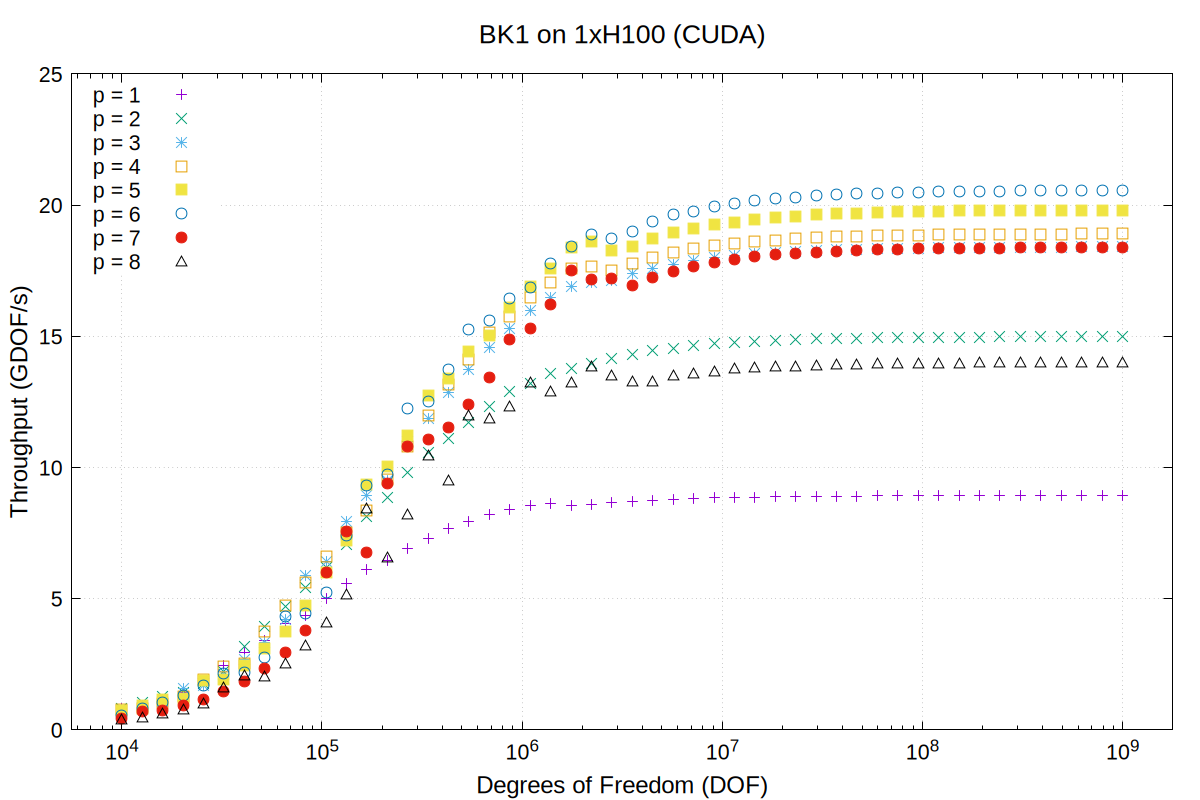
\includegraphics[width=0.8\textwidth]{BK1_1}
\caption{BK1 performance results on Nvidia H100 GPU with CUDA programming model. Various polynomial orders are tested, and saturation of hardware resources is visible after $10^6$ degrees of freedom. Polynomial order 1 performs the worst due to under-occupation of the single warp. {\color{red} Have not placed the two figures side-by-side as requested as labels are already too small. Please provide new figures.}}
\label{fig:BK1_1}
\end{figure}
\begin{figure}
\centering
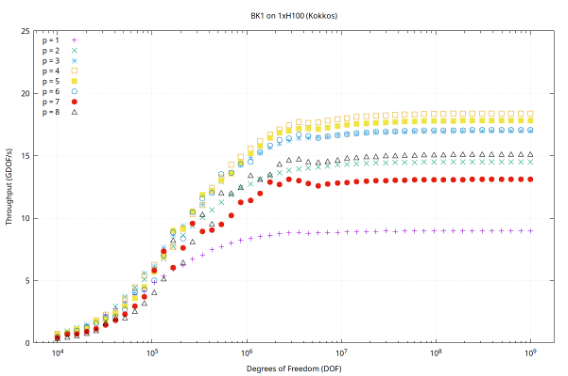
\includegraphics[width=0.8\textwidth]{BK1_2}
\caption{BK1 performance results on an NVIDIA H100 GPU using the Kokkos library. The same test conditions and optimization techniques as in Figure 1 were applied. Kokkos attains nearly 90\% of the performance delivered by CUDA.}
\label{fig:BK1_2}
\end{figure}

{\bf BK5.} Unlike the multiple polynomial order evaluations in the BK1 test cases, we analyzed the kernels with a fixed cubic polynomial order (p=3) and templated quadrature points. Using templates shifts certain computations from runtime to compile-time, allowing the compiler to apply optimizations. As a result, templated implementations are often significantly faster, in most cases improving performance by 30\% at least, compared to their runtime counterparts.

Both CUDA and Kokkos kernels were implemented with three-dimensional thread blocks and a simple data mapping approach, where each thread operates on a single data entry. The total number of degrees of freedom (DOF) in this test case is 27 million. Kernel performance values were measured by NVIDIA Nsight Compute. In these measurements, both CUDA and Kokkos executions completed in 0.71 ms, showing identical performance. Nsight Compute reported an arithmetic intensity of 1.97 FLOP/byte, which places these kernels in the memory-bound region of the roofline model for the H100 GPU. The achieved performance was 5.7 TFLOPs, compared to the hardware limit of 6.6 TFLOPs at this arithmetic intensity. This corresponds to 86\% of peak bandwidth utilization (2.88 TB/s out of 3.2 TB/s). The kernels also achieved 75\% occupancy, and register usage per thread was identified as the primary limiting factor.

Overall, the results demonstrate that both CUDA and Kokkos BK5 implementations deliver near-optimal performance on the H100, efficiently exploiting available memory bandwidth and achieving performance levels very close to the hardware limits.


\section{Improvement of pre-exascale modules of the deal.II library}

Work package 1.2 focuses on enhancing the existing modules of the deal.II
library to prepare them for the challenges of exascale computing. This includes
several key activities: 
\begin{itemize}
    \item Improving the gmsh API to support large-scale;
    \item Developing a generalized interface for coupling operators, which
    is fundamental for multiphysics and multiscale simulations, including methods
    for conforming and non-conforming grids and non-local coupling techniques;
    \item Enhancing the reduced-order modeling (ROM) capabilities of deal.II,
    implementing algorithms for data analysis and reduced-order geometric modeling;
    \item Integrating low-rank approximation methods within deal.II, including
    low-rank and hierarchical low-rank solvers and preconditioners to tackle
    large-scale computational problems;
    \item Developing block preconditioners for coupled problems, which are
    essential for the stability and efficiency of simulations.
\end{itemize}
 
The overall objective is to improve the pre-exascale functionalities of deal.II,
making it an even more robust and efficient library for a wide range of
scientific and engineering applications aiming for the use of exascale
computers.

\subsection{Extension of current gmsh API for exascale simulations}
    The key researcher in this task is a postdoc researcher, Dr. Devi Raksha, who
    has been hired on the project, and will start her position in April 2025.
    The task is to extend the gmsh API to support large-scale simulations, with
    a focus on biomedical applications, and to improve the gmsh deal.II
    interface to enable the generation and handling of large-scale meshes.

    The task has not been started yet, and it is postponed to the second
    semester of the project.

\subsection{Generalized Interface for Coupling Operators in deal.II}
    \subsubsection{Objectives and Planned Activities (Task WP1.2.2)}

    The objective of this task is to develop a generalized interface for
    coupling operators in deal.II, which is essential for multiphysics and
    multiscale problems. The focus is on two different types of coupling:
    \begin{itemize}
        \item Coupling between different physical processes, such as fluid-structure interaction or heat transfer in porous media;
        \item Coupling between different discretization schemes, including
        non-matching and non-overlapping discretizations.
    \end{itemize}

    This subtask was supposed to start on the second semester of the project,
    but an early version of the generalized interface has been developed and
    merged into the deal.II repository in April 2024, before the official start
    of the dealii-X project, making it more convenient to start the development
    of the rest of this task in the first semester.

    The developed approach encompasses two main aspects: a high-level interface
    for defining coupling operators and a low-level interface for implementing
    efficient evaluation of coupled bilinear forms (on possibly non-matching or
    non-nested grids). The high-level interface enables the computation of
    abstract bilinear forms for coupling between geometric entities, supporting
    various kernels and use cases like BEM and bulk-surface coupling. The low
    level interface needs to be flexible enough to allow the use of different
    discretization schemes, including non-conforming discretizations, and
    possibly different parallel distributions of the meshes.

    \subsubsection{Implementation Details} 

    The two pull requests, ``FECouplingValues''
    (\url{https://github.com/dealii/dealii/pull/15773}) and
    ``FEValuesViews::RenumberedView''
    (\url{https://github.com/dealii/dealii/pull/15819}), directly address the
    objective of developing a ``Generalized interface for coupling operators in
    deal.II'', as outlined in Work Package 1.2.2 of the dealii-X project, by
    providing the high level interface discussed in the introduction.

    Pull request \#15773 introduces a new class called `FECouplingValues`, specifically designed for the computation of general coupling operators. The primary goal of this class is to enable the computation of abstract bilinear forms of the type:
    $$ \int_{T_1} \int_{T_2} K(x_1, x_2) f(x_1) g(x_2) \, dT_1 \, dT_2, $$ where
    $T_1$ and $T_2$ represent two arbitrary sets (cells, faces, edges, or their
    combinations), and $K$ is a coupling kernel (potentially singular). The
    class is designed to support various types of kernels $K$. The pull request
    includes several tests demonstrating how the class can be used for different
    types of coupling:
    \begin{itemize}
        \item Coupling for Boundary Element Methods (BEM);
        \item As a replacement for `FEInterfaceValues`, integrating
        discontinuous Galerkin flux terms;
        \item For bulk-surface coupling computations.
    \end{itemize}


    Pull request \#15819 introduces the class `FEValuesViews::RenumberedView`.
    This component was developed as part of the work for \#15773 and is intended
    for use by `FECouplingValues`. `RenumberedView` allows the creation of a
    reordered view of an `FEValuesBase` object, where both degrees of freedom
    and quadrature points are renumbered according to provided renumbering
    vectors.

    In summary, these two pull requests jointly implement the "Generalized interface for coupling operators in deal.II" envisioned in WP1.2.2:
    \begin{itemize}
        \item `FECouplingValues` provides the framework for defining and
        computing general coupling operators between different geometric
        entities and discrete spaces. This addresses the need for a versatile
        interface to manage various coupling techniques, including methods for
        non-matching grids and non-local coupling.
        \item `FEValuesViews::RenumberedView` provides a fundamental tool for managing the correspondence (or lack thereof) between the degrees of freedom and quadrature points of the different spaces being coupled via `FECouplingValues`.
    \end{itemize}

    The integration of these two functionalities into the deal.II library
    provides users with powerful and flexible tools to tackle complex coupling
    problems essential for the multiphysics and multiscale simulations at the
    core of the dealii-X project.

    The two pull requests were merged into the main deal.II repository on April
    11, 2024, and included in the Release 9.6 milestone, before the official
    start of the dealii-X project. As part of the WP1.2 tasks, a biologically
    relevant application that uses the new functionality is being developed and
    will be integrated in the deal.II repository as a new tutorial program. The
    tutorial will demonstrate the use of the new `FECouplingValues` class for
    the computation of a bulk-surface coupling operator.

    A low level interface for coupling operators has been developed and merged
    into the deal.II repository in pull request \#17919, which introduces a new
    abstract base class `MGTwoLevelTransferBase` to enable non-nested multigrid
    transfers. The primary goal of this class is to generalize the interface for
    managing transfers between non-nested grids, which is a crucial step towards
    addressing the challenges of coupling operators on non-matching grids. 

    The `MGTwoLevelTransferBase` class provides a flexible framework for
    implementing matrix-free transfer operators between different levels of a
    multigrid hierarchy. This development aligns with the objectives of WP1.2.2,
    as it contributes to the creation of a generalized interface for coupling
    operators in deal.II. Additionally, the techniques developed for non-nested
    multigrid transfers could offer valuable insights and algorithms for
    tackling coupling problems on non-matching grids in more general contexts.

    The implementation of this low-level interface is expected to enhance the
    scalability and efficiency of multigrid methods in deal.II, particularly for
    applications involving complex grid hierarchies or non-conforming
    discretizations. This work also complements the high-level interface
    provided by `FECouplingValues`, creating a comprehensive toolkit for
    addressing a wide range of coupling and multigrid challenges in the dealii-X
    project. The work has been submitted, and is currently under review. A
    preprint is available at ~\cite{FederEtAl2024b}.

   A tutorial program that illustrates the use of the non-nested multigrid
   transfer has been proposed and is currently under review in the deal.II
   library
    \url{https://github.com/dealii/dealii/pull/17919}.


\section{Polygonal Discretization Methods}

 The dealii-X project Work Package 1.3, lead by the SISSA team, will deliver an experimental module enhancing the
deal.II library with the capability to perform efficiently polygonal discretization, that is numerical methods based on general polygonal and polyhedral meshes.% in place of standard simplicial and hexahedral meshes. 

\subsection{Objectives and Planned Activities (Task WP1.3.1 and WP1.3.2)}

%The primary objective of WP1.3 is the development of a polygonal discretization module within the deal.II library. 
The deal.II library currently
supports a wide range of finite element methods, defined on standard simplicial
and hexahedral meshes, but does not support polygonal and polyhedral (\emph{polytopic}) meshes.
The primary objective of WP1 is the development of a polygonal
discretization module within the deal.II library. The module is designed to be integrated into the deal.II library, and its integration is expected to be completed by the end of the project.

This task requires the development of the basic data structure for polytopic meshes obtained by agglomeration of standard deal.II meshes and the exploitation of such data structure for the implementation of polygonal discretizations.


 \subsection{Progress and Current Status}

The preliminary version of the polygonal discretization module developed within the first six months of the project was made available at https://github.com/fdrmrc/Polydeal.
The module has since been extensively tested and parallelised. 
Milestone M5 has been reached and deployed as deliverable D1.5 (cf. the specific report for more details). The milestone was set to establish the parallel implementation of polygonal discretization methods. The deliverable provides a tutorial program on polygonal discretizations, showcasing the implementation of these methods for the solution of a basic model problem. Aside from the tutorial, a series of problems and tests have been run, confirming the validity and robustness of the approach for the solution of problems in the dimension-independent setting. In particular, the polytopic discontinuous Galerkin methods have been implemented for the solution of a series of benchmark problems, including fluid mechanics and electrophysiology.


{\bf Fluid mechanics.}
The polytopic discontinuous Galerkin method has been extended to the solution of fluid mechanics boundary value problems with the analysis of the method for the solution of the Oseen problem. This required a new analysis which has been carried out for the $hp$-version of the method, hence permitting arbitrarily high-order implementations. Both stabilised equal order $(\mathcal{P}_k,\mathcal{P}_{k})$ and pressure lower-order $(\mathcal{P}_k,\mathcal{P}_{k-1})$ versions have been analysed. 
New working examples implementing the new method have been committed by the SISSA team within the examples suits of the {\em polydeal} repository \url{https://github.com/fdrmrc/Polydeal}.
% https://github.com/fdrmrc/Polydeal/blob/main/examples/darcy_stokes.cc
Preliminary results show that the polytopic discontinuous Galerkin (polyDG) is achieving the optimal convergence rate when applied to the Oseen problem. Using the \emph{polydeal} data structure, a sequence of polygonal meshes obtained by agglomeration of a single fine quadrilateral mesh has been created, see Figure~\ref{fig:metis}. The corresponding results shown in Table~\ref{tab:meshes} display the corresponding convergence rate achieved by the polyDG method solving a model problem for the Oseen equation with variable coefficients.
\begin{figure}[!htb]
\centering
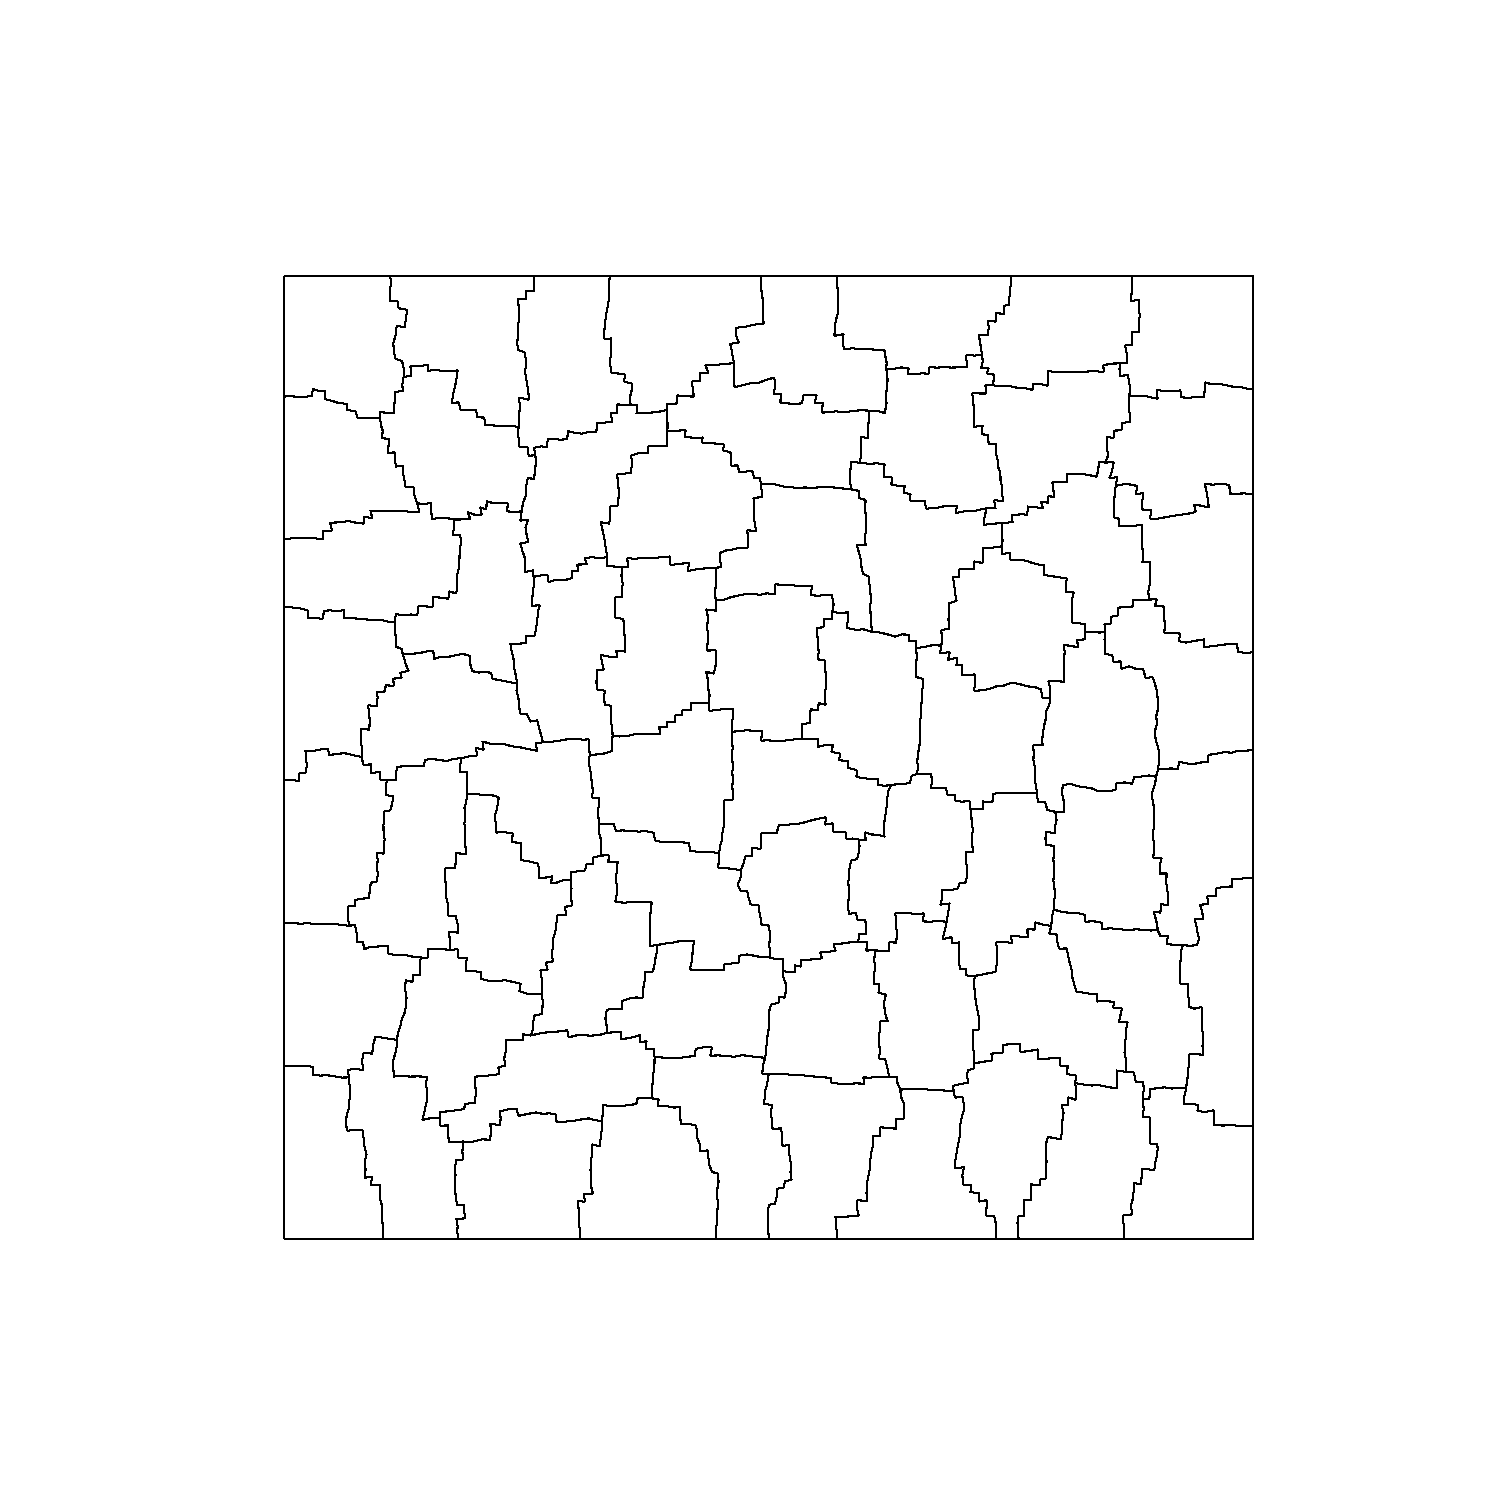
\includegraphics[height=0.3\linewidth]{metis_level3}
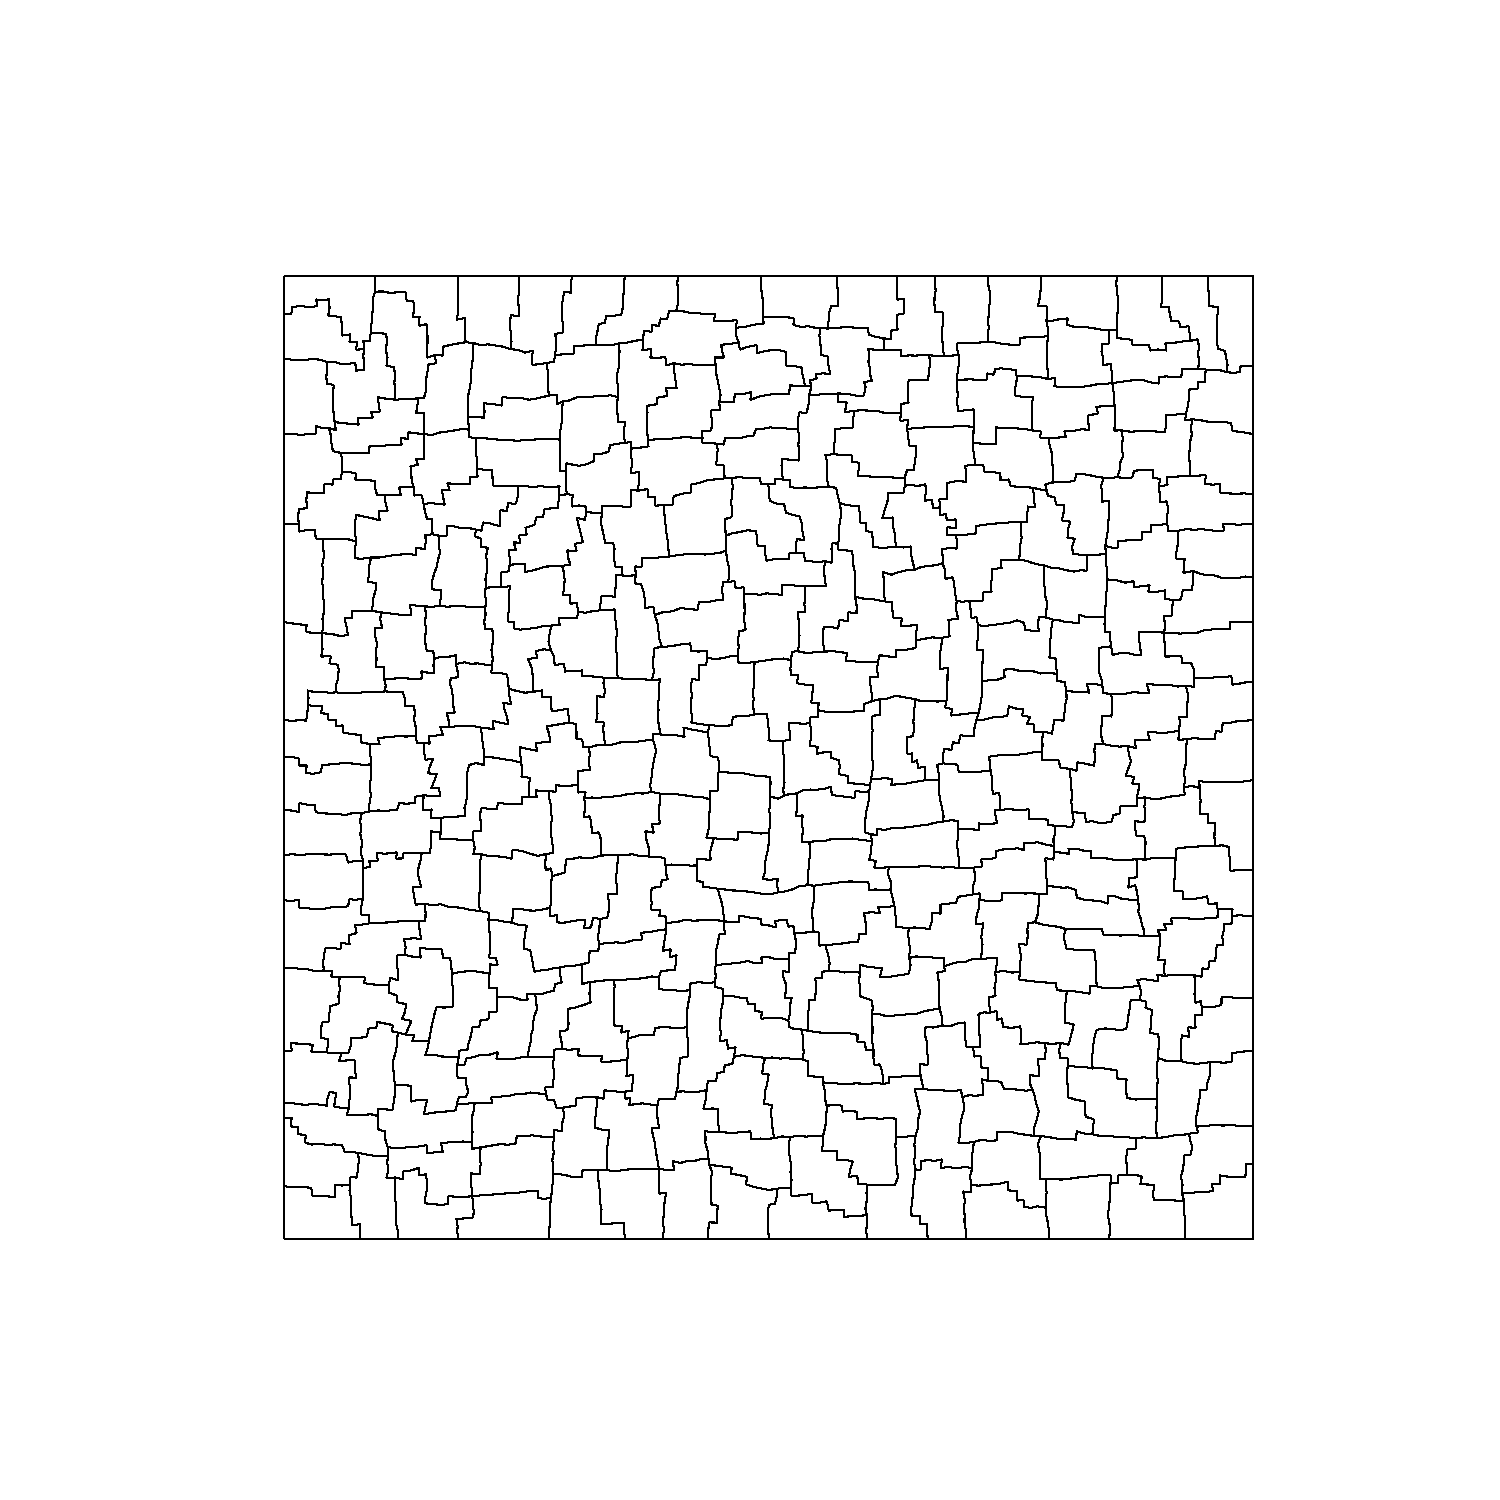
\includegraphics[height=0.3\linewidth]{metis_level4}
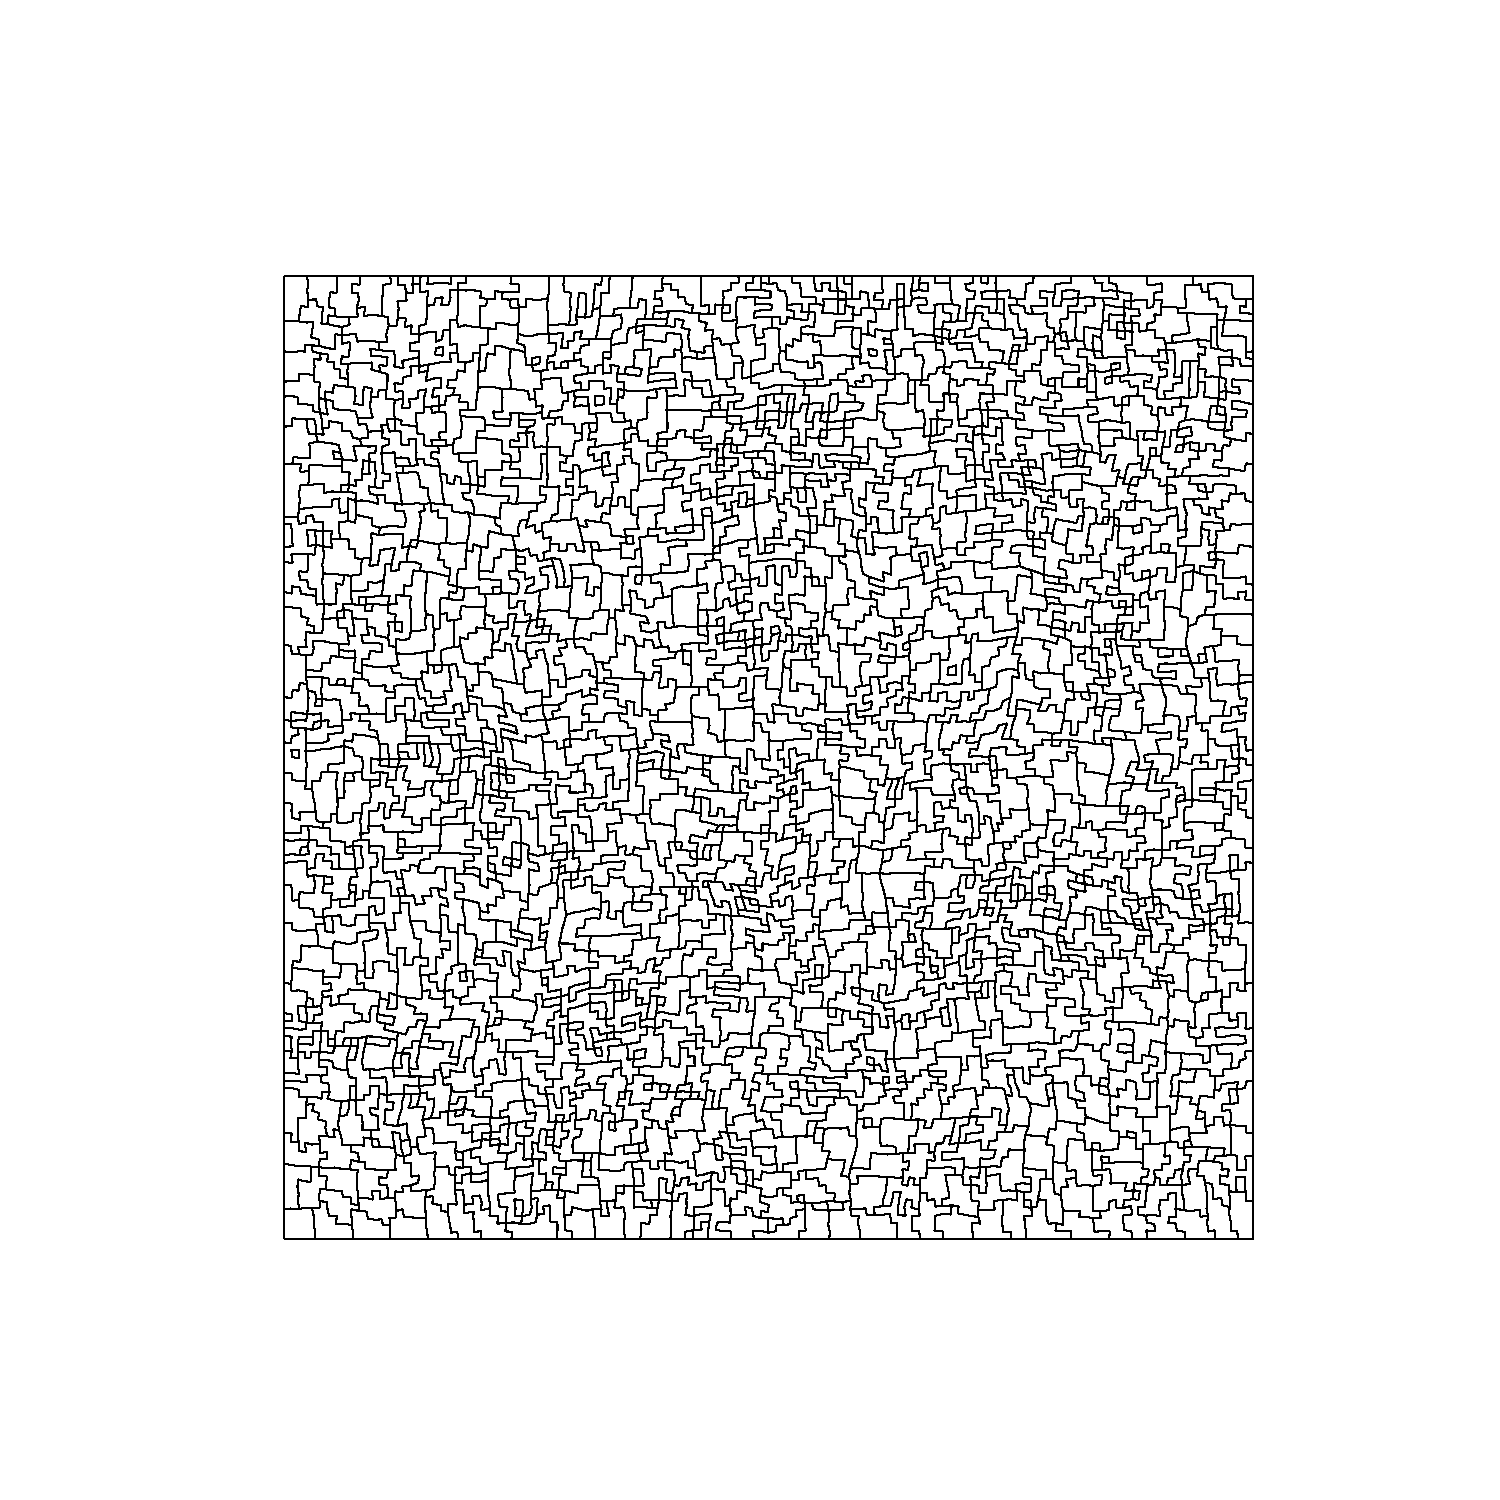
\includegraphics[height=0.3\linewidth]{metis_level5}
\label{fig:meshes}
\caption{Three subsequent levels of the meshes obtained by METIS-based agglomeration of an underlying fine quadrilateral mesh.}
\end{figure}
\begin{table}[!ht]\centering
\caption{$\normdg{(\cdot,\cdot)}_{\star}$ norms of errors and convergence orders for the test problem on three different meshes with $Re=1$. {\color{red} TABLE IN PROGRESS!}}
\label{tb1}
{\small
\begin{tabular}[c]{cc|cccccc}\hline\hline
&\multirow{2}*{Level}
&\multicolumn{2}{c}{ Mesh 1 }
&\multicolumn{2}{c}{ Mesh 2 }
&\multicolumn{2}{c}{ Mesh 3 }
 \\ \cline{3-8}
&&$\normdg{({\bf e}_{\vecu},e_p)}_{\star}$&order&$\normdg{({\bf e}_{\vecu},e_p)}_{\star}$&order
&$\normdg{({\bf e}_{\vecu},e_p)}_{\star}$&order\\ \hline
\multirow{4}*{$\mathcal{P}_2$-$\mathcal{P}_2$}
&4 &8.32E-00&1.85&6.75E-00&2.03&7.69E-00&1.86\\
&5 &2.17E-00&1.94&1.76E-00&1.94&2.46E-00&1.64\\
&6 &4.54E-01&2.25&4.91E-01&1.84&6.50E-01&1.92\\
&7 &8.87E-02&2.36&1.17E-01&2.08&1.17E-01&2.48\\
\hline
\multirow{4}*{$\mathcal{P}_3$-$\mathcal{P}_2$}
&4 &1.20E-00&2.63&1.14E-00&2.59&1.16E-00&2.70\\
&5 &1.73E-01&2.79&1.50E-01&2.93&2.14E-01&2.44\\
&6 &1.99E-02&3.13&2.07E-02&2.85&3.21E-02&2.73\\
&7 &1.98E-03&3.32&2.68E-03&2.95&2.68E-03&3.58\\
\hline\hline
\end{tabular}}
\label{tab:oseen}
\end{table}
A publication presenting both the new sharp a priori analysis of the discontinuous Galerkin method for the Oseen problem as well as numerical experiments validating the approach for both the solution of the Oseen and coupled Darcy-Stokes problems is under preparation. It will be submitted to a top numerical analysis journal within the next semester.

{\bf Electrophysiology.}
A novel multilevel preconditioning strategy has been developed and implemented for solving the monodomain equation in cardiac electrophysiology using high-order Discontinuous Galerkin methods. The approach centers on the R*-tree spatial data structure to automatically generate coarse grid hierarchies from predetermined fine meshes, in order to create agglomerated polytopic elements by traversing tree levels. The mathematical framework employs inherited bilinear forms where coarse operators are constructed via Galerkin projection $A_{l+1} = (P_{l+1}^l)^T A_l P_{l+1}^l$, avoiding the computational expense of assembling operators on polytopic elements. The monodomain equation $\frac{\partial u}{\partial t} + \mathcal{I}_{ion}(u,\mathbf{w}) - \nabla \cdot (\mathbb{D} \nabla u) = \mathcal{I}_{app}$ is discretized using Symmetric Interior Penalty DG with semi-implicit time stepping, treating diffusion implicitly and reaction terms explicitly.

The C++ implementation builds upon the \url{https://github.com/fdrmrc/Polydeal} library, based on deal.II. The agglomeration algorithm demonstrates excellent scalability, maintaining load balance across 128 to 1024 processors even on realistic three-dimensional cardiac geometries. Memory requirements scale favorably due to the matrix-free implementation of prolongation and restriction operators.

Numerical experiments, performed on two different test cases, demonstrate consistent superior performance compared to algebraic multigrid preconditioning. For polynomial degrees ranging from $p=1$ to $p=5$, the method achieves lower iteration counts across all test cases, as reported in Figure \ref{fig:iterates_level_3D_monodomain_p_2}. The advantage becomes more pronounced with increasing polynomial degree. The method also exhibits minimal dependence on the number of multigrid levels. The coarsening algorithm maintains geometric quality while preserving the spatial locality of agglomerated elements, resulting in well-conditioned coarse grid operators. The preconditioner integrates V-cycle multigrid with Chebyshev smoothers, using eigenvalue estimates computed via Lanczos iterations.

\begin{figure}[!htb]
    \centering
    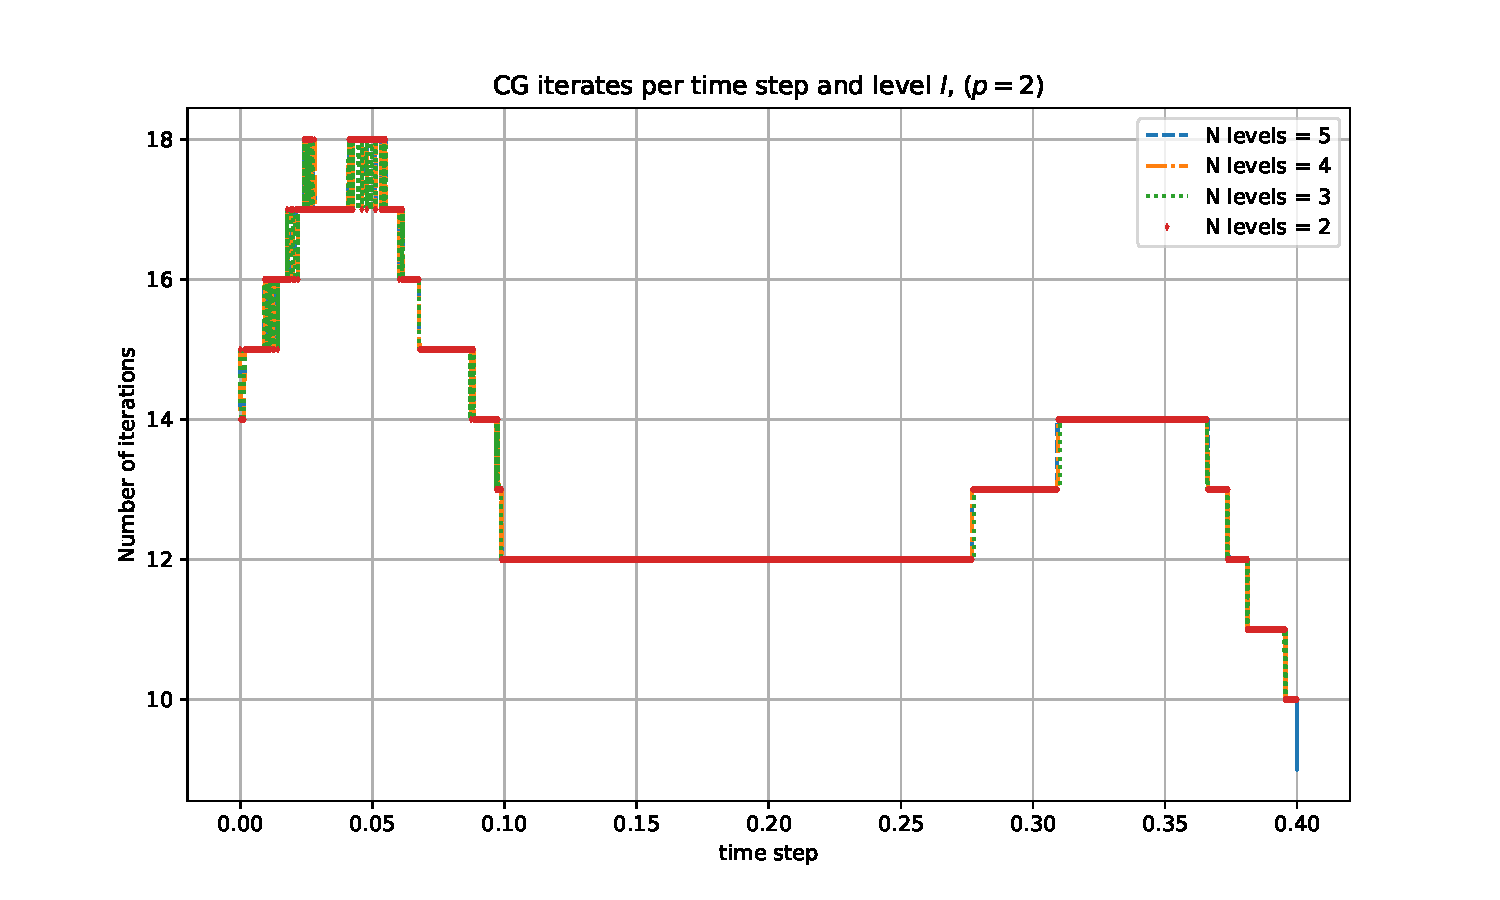
\includegraphics[width=0.9\textwidth]{l_p_2.pdf}
    \caption{Number of CG iterations per time step for the monodomain problem in an idealized ventricle test case with $p=2$ and different number of levels.}
    \label{fig:iterates_level_3D_monodomain_p_2}
\end{figure}


 \subsection{Challenges and Future Plans}

Before integration into the deal.II library, additional testing and generalization are necessary to demonstrate the potential of polygonal discretization in solving the same range of models currently supported by standard finite elements. Moreover, further work on efficient implementation is required to fully exploit the complexity-reduction capabilities of these methods. This effort will include, for example, the development of advanced solvers, such as multigrid techniques and automated mesh adaptivity algorithms, which constitute the next phase of the project.


\section{Integration of PSCToolkit into deal.II (WP1.4)}
    \subsection{Objectives and Planned Activities}
        The primary objective of WP1.4 is to integrate the PSCToolkit (Parallel Sparse Computing Toolkit) into the deal.II library. This integration aims to leverage GPU computing to enhance performance and develop efficient preconditioners for multiphysics problems. PSCToolkit provides advanced routines for sparse matrix operations optimized for GPU architectures, which are critical for large-scale simulations.

        Planned activities include:
        \begin{itemize}
            \item Developing a GPU-accelerated interface for PSCToolkit within deal.II;
            \item Implementing efficient preconditioners tailored for multiphysics problems;
            \item Benchmarking the performance of the integrated toolkit on exascale systems.
        \end{itemize}

        \subsection{Progress and Current Status}
        Initial efforts have focused on designing the interface between PSCToolkit and deal.II's existing data structures. A pull request has been opened in the deal.II repository to support detection and linkage with the PSBLAS library (one of the two core libraries identified for interfacing PSCToolkit with deal.II; the other is AMG4PSBLAS, whose integration will follow in a subsequent pull request) \url{https://github.com/dealii/dealii/pull/18199}. A prototype of the interface has been planned in collaboration with the MUMPS team to ensure seamless integration with deal.II's current data structures of both interfaces.

        Several enhancements have been made to the PSCToolkit library itself to facilitate its integration with external libraries (such as deal.II), including:
        \begin{itemize}
            \item Fine control and tuning of compile definitions to simplify the detection of the library and its components, including support for external libraries, ensuring compatibility at linking time with deal.II and its dependencies;
            \item Adding support for CMake to streamline integration with external libraries;
            \item Exporting the library's macro definitions in a dedicated header file to simplify detection of the library and its components, regardless of the build system used;
            \item Adding PSBLAS to the Spack package manager to simplify the installation of the library and its dependencies.
        \end{itemize}

        \subsection{Challenges and Future Plans}

        The integration of PSCToolkit into deal.II is still in its early stages, requiring careful planning to ensure compatibility and performance. The primary challenge lies in ensuring that the interface between PSCToolkit and deal.II is robust, efficient, and seamlessly communicates with existing deal.II data structures without introducing additional ones. This challenge stems from the proliferation of slightly incompatible data structures in existing external linear algebra packages integrated with deal.II, which has led to significant maintenance efforts and user confusion. Addressing this issue is a key focus to ensure a streamlined and user-friendly integration.

\section{Integration of MUMPS Solver into deal.II (WP1.5)}
    \subsection{Objectives and Planned Activities}
    WP1.5 aims to integrate the MUMPS (Multifrontal Massively Parallel Sparse) solver directly into deal.II. This task focuses on enabling its use in multigrid methods and exploring advanced techniques such as low-rank approximations and mixed-precision computations to enhance solver efficiency.

    Planned activities include:
    \begin{itemize}
        \item Developing a direct interface between deal.II and MUMPS;
        \item Implementing low-rank approximation techniques to reduce computational costs;
        \item Exploring mixed-precision strategies to optimize performance on modern hardware.
    \end{itemize}

    \subsection{Progress and Current Status}
    A preliminary interface for MUMPS was present in the deal.II library until
    version 9.2. Such interface had been removed, in favor of using MUMPS
    through external linear algebra packages such as PETSc and Trilinos.
    
    A careful planning of the interface between deal.II and MUMPS is currently
    ongoing, with the goal of ensuring that the interface is robust and efficient,
    and that it seamlessly communicates with existing deal.II data structures, extending, integrating, and modernizing the former MUMPS interface in deal.II. An initial pull request
    has been opened in the deal.II repository to support detection and linkage
    with the MUMPS library, reverting the removal of the MUMPS interface in deal.II, and re-introducing the original MUMPS interface, including some simple tests to ensure that the interface is working correctly. The pull request is available at
    \url{https://github.com/dealii/dealii/pull/18255}.
    
    \subsection{Challenges and Future Plans}

    The integration of MUMPS into deal.II is currently working only with the
    serial version of the deal.II data structures, and it is still in its early
    stages, requiring careful planning to ensure compatibility and performance.
    Similarly to what has been discussed with the PSBLAS library, the primary
    challenge lies in ensuring that the interface between MUMPS and deal.II is
    robust, efficient, and seamlessly communicates with existing deal.II data
    structures. Ensuring compatibility and avoiding redundant data structures is
    crucial to streamline integration and reduce maintenance efforts.

\bibliographystyle{abbrv}
%\bibliography{../common/bibliography.bib}
\bibliography{bibliography.bib}
    
%\label{MyLastPage}


\end{document}
